% This file was created with tikzplotlib v0.10.1.post13.
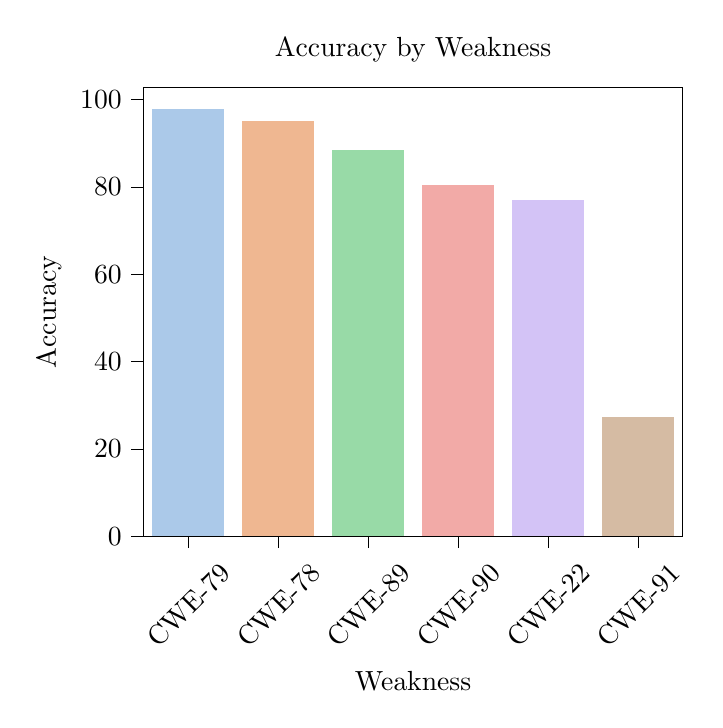
\begin{tikzpicture}

\definecolor{burlywood239183145}{RGB}{239,183,145}
\definecolor{darkgrey176}{RGB}{176,176,176}
\definecolor{darkslategrey66}{RGB}{66,66,66}
\definecolor{lightgreen152218167}{RGB}{152,218,167}
\definecolor{lightpink242170167}{RGB}{242,170,167}
\definecolor{lightsteelblue171201233}{RGB}{171,201,233}
\definecolor{tan213187163}{RGB}{213,187,163}
\definecolor{thistle211195246}{RGB}{211,195,246}

\begin{axis}[
tick align=outside,
tick pos=left,
title={Accuracy by Weakness},
unbounded coords=jump,
x grid style={darkgrey176},
xlabel={Weakness},
xmin=-0.5, xmax=5.5,
xtick style={color=black},
xtick={0,1,2,3,4,5},
xticklabel style={rotate=45.0},
xticklabels={CWE-79,CWE-78,CWE-89,CWE-90,CWE-22,CWE-91},
y grid style={darkgrey176},
ylabel={Accuracy},
ymin=0, ymax=102.687224669604,
ytick style={color=black}
]
\draw[draw=none,fill=lightsteelblue171201233] (axis cs:-0.4,0) rectangle (axis cs:0.4,97.7973568281938);
\draw[draw=none,fill=burlywood239183145] (axis cs:0.6,0) rectangle (axis cs:1.4,95.0248756218905);
\draw[draw=none,fill=lightgreen152218167] (axis cs:1.6,0) rectangle (axis cs:2.4,88.4173297966401);
\draw[draw=none,fill=lightpink242170167] (axis cs:2.6,0) rectangle (axis cs:3.4,80.3455723542117);
\draw[draw=none,fill=thistle211195246] (axis cs:3.6,0) rectangle (axis cs:4.4,76.9230769230769);
\draw[draw=none,fill=tan213187163] (axis cs:4.6,0) rectangle (axis cs:5.4,27.2727272727273);
\addplot [line width=0.9pt, darkslategrey66]
table {%
0 nan
0 nan
};
\addplot [line width=0.9pt, darkslategrey66]
table {%
1 nan
1 nan
};
\addplot [line width=0.9pt, darkslategrey66]
table {%
2 nan
2 nan
};
\addplot [line width=0.9pt, darkslategrey66]
table {%
3 nan
3 nan
};
\addplot [line width=0.9pt, darkslategrey66]
table {%
4 nan
4 nan
};
\addplot [line width=0.9pt, darkslategrey66]
table {%
5 nan
5 nan
};
\end{axis}

\end{tikzpicture}
